\chapter{New Framework}

\section{Assuming chaos (ergens anders)}

One of the most important features about our framework is that it assumes chaos. The meaning of this is three-fold:

FOUNDATION

\begin{itemize}

\item All instances are considered different authors until proven otherwise. ...

\item No decision is made permanent

\item Any information is considered partial information. ...

\item A constantly changing input asks for a constantly changing output. ... % meer aan de kant van de omgeving, het leven gaat door :p

\item The stream of informaton is endless. ... % meer aan de kant van het framework, nieuwe plugins

\end{itemize}

\section{Why the first approach needed a complete overhaul}

%The first approach was all about trying to solve a complex problem with a simple solution. We sticked with this approach as long as we could. As we started to see more and more flaws, we decided that the framework needed a complete overhaul. The following paragraphs try to explain these flaws in short.

% verwijs naar waar de problemen worden opgelost, en zeg dat je de problemen nog zal "recapituleren"

% in afkortingen vermelden van verwezen wordt naar eerste versie framework als Fv1

\paragraph{The flow of data} %A logical flow of data in a system with this much data to process is of primary importance. In Fv1, several components (that are part of building the solution) did not comunicate directly with each other. All communication is "relayed" through the database. This puts enormous unnecessary load on out database.

\paragraph{Scalability} %The more instances in the cluster, the more queries to the dabase to retreive the information to do the job ... Not easy to have data flow dependencies (also communicate via database?)

\paragraph{The right tool for the job} %Mysql vs Graphdb

\paragraph{Static system in a dynamic environment} %The academic world is a very dynamic one. Researchers are constantly publishing, moving from one location to another and putting new information about themselves on the internet. The increasing amount of places on the web to find this information only makes our environment more sensitive to change in the real world. It is clear that a static solution does not satisfy our needs. Fv1

\paragraph{Performance} %snapshot vs incremental. In a dynamic env snapshot is constantly intensive. Incremental is only once intensive. (combine with static)

\section{New foundation: Distributed Pipes and Filters}

introduction

\subsection{Small and Simple Core}

\paragraph{Pipes and Connectors} +figuur

\paragraph{Connections} % niet beginnen over async stuff, later "gebruiken"

\subsection{Some useful pipes}

\paragraph{Merge and Split}

\paragraph{Filter}

\subsection{Extending to fit our needs}

\paragraph{Pipes with memory} 

\paragraph{Flow enrichment}

\paragraph{Parsers}

\paragraph{Asynchronous connections}

\paragraph{Locking}

\section{Practical applications}

\subsection{Dependency Resolution}

\subsection{Concurrent, incremental Clustering}

Clustering is a very important step in building towards a solution. Each new flow of information indirectly leads to a clustering operation. Acquiring new information triggers rules which on their turn yield similarities. These similarities change the balance between clusters. In the worst case, an expensive rebalancing procedure is necessary.

It is obvious that processing similarities is something that will be executed very frequently (numbers?). The combination of the enormous amount of similarities and their expensive processing requires us to make this process as streamlined and efficient as possible. The clustering algorithm as explained in [REF] leads to a first, na\"ive implementation approach. Rethinking the absolute needs of the clustering algorithm then leads to a second approach that benifits greatly of the foundations of our framework.

\paragraph{In-graph implementation} The most simple solution one can think of is to maintain the ICW and OCW for every vertex in the vertex itself. The adjacency matrix would implicitly be defined by the edges between two nodes in the similarity plane. This technique has two main drawbacks:

\begin{enumerate}
\item A lot of load would be pushed to the database.
\item There would be a need for several concurrency control mechanisms/
\end{enumerate}

If clustering could be executed without the use of the database in an efficient manner, it would be preferrable. After all it is in our best interest to take as much load as possible away from the database because it is much more difficult to scale than our pipes and filters architecture. Besides, the similarity ``meta''-plane is not something that should be queried from our end-user application. The users are interested in the result of the clustering, not the way it got there.

In the case of similarities being processed in parallel, we need to pay some extra attention. We do not want that the clustering mechanism inflicts race conditions and, by consequence, inconsistencies on the graph.


\paragraph{As a stateful pipe}

\begin{algorithm}
\caption{!!!}
\label{mincutgusfield}
\begin{algorithmic}
\STATE \textbf{lock} $I_1,I_2$
\IF{cluster($I_1$) == cluster($I_2$)}
  \STATE \textbf{watch} $C_1,C_2$
  \STATE \textbf{unlock} $I_1,I_2$
  \STATE \textbf{process(intra-cluster)}
\ELSE
  \STATE \textbf{lock} $C_1,C_2$
  \STATE \textbf{unlock} $I_1,I_2$
  \STATE \textbf{process(inter-cluster)}
  \STATE \textbf{execute}
  \STATE \textbf{unlock} $C_1,C_2$
\ENDIF
\end{algorithmic}
\end{algorithm}

\begin{figure}[htbp]
	\centering
		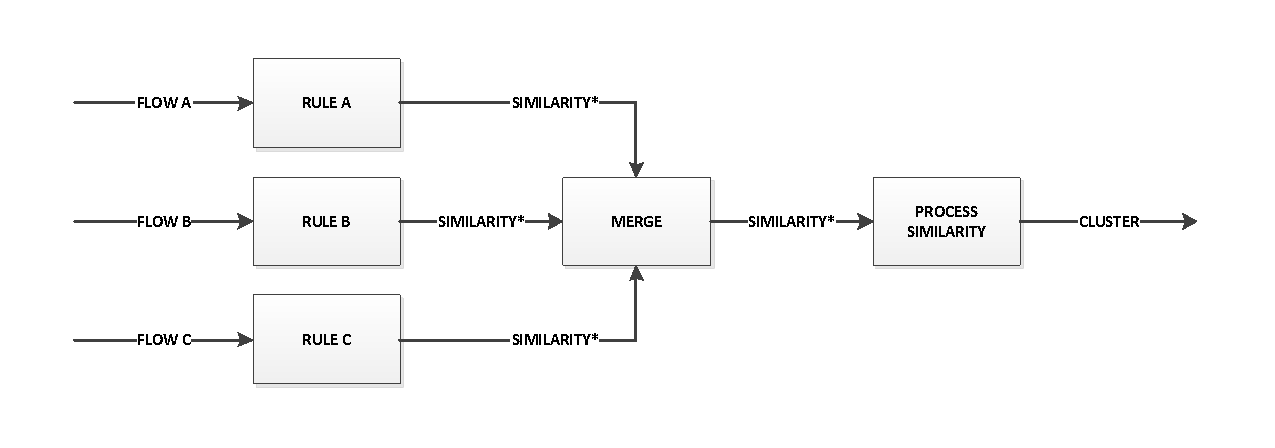
\includegraphics[width=1\textwidth]{fig/clusteringpipe}
	\caption{Clustering flow}
	\label{fig:clusteringpipe}
\end{figure}

\subsection{Assignment of e-mail addresses}